\chapter{Descripción}
\label{cap:descripcion}

% ═════════════════════════════════════════════════════════════════════════════
\section{Contexto y necesidades detectadas}

DePaso se define como una plataforma digital (app móvil) de logística urbana colaborativa diseñada para conectar clientes con transportistas y mitigar las ineficiencias de la última milla en el AMBA. El proyecto aborda de forma directa las necesidades de los actores clave afectados por el escenario logístico urbano actual:

\begin{itemize}[leftmargin=2em]
	\item \textbf{Clientes particulares}: enfrentan costos elevados y falta de opciones para envíos pequeños o medianos. A esto se suman la poca flexibilidad horaria y la ausencia de seguimiento en tiempo real, que genera incertidumbre sobre la llegada de los pedidos.
    \item \textbf{PyMEs y comercios}: al no disponer de flota propia, contratar un flete dedicado les exige pagar un vehículo completo para realizar envíos pequeños o medianos, limitando los márgenes en cada operación. \nuevo{A esto se suma que la incertidumbre respecto del precio y la disponibilidad de un flete les dificulta comprometerse de antemano con sus propios clientes: no pueden anunciar una tarifa de envío fija ni ofrecer, cuando la operación lo justifica, un envío sin cargo como recurso comercial, porque desconocen con anticipación cuánto les costará conseguir el flete ni si lo conseguirán a tiempo. Esa falta de previsibilidad las deja en desventaja frente a competidores de mayor escala que sí pueden sostener esas condiciones, y las obliga a absorber el riesgo o el costo de esa incertidumbre, o directamente a resignar la venta. Esta dificultad no es anecdótica: en un relevamiento regional a más de 2.000 MiPyMEs de Argentina, Brasil, Colombia y México, el 44~\% señaló el costo de entrega o devolución como uno de los principales obstáculos para vender en línea \parencite{ICC2024}.} Por otra parte, contar con un sistema de envíos de rango más amplio les permitiría llegar a clientes que no pueden retirar en el local por cuestiones de tiempo o movilidad.
    \item \textbf{Transportistas ocasionales}: miles de personas realizan trayectos cotidianos (al trabajo, por trámites o por estudio) cuyo costo recae íntegramente sobre estas. Cuentan con espacio disponible en sus vehículos, el cual puede resignificarse en una oportunidad de ingreso. Las plataformas actuales exigen exclusividad y disponibilidad de tiempo completo, condiciones incompatibles con un empleo de oficina o una rutina personal.
    \item \textbf{Personas que se dedican al transporte de carga}: trabajan con una demanda irregular, con picos de trabajo seguidos de períodos sin ingresos. La falta de una plataforma estructurada para conectar con clientes limita su capacidad de crecimiento y profesionalización; acceder a una les permitiría captar nuevas oportunidades de negocio y sostener la demanda de forma constante.
	\item \textbf{Entorno urbano}: el esquema de viajes dedicados incrementa considerablemente los vehículos en circulación, lo que genera congestión y emisiones de CO\textsubscript{2} que podrían evitarse reduciendo el número de vehículos utilizados para logística.
\end{itemize}

La propuesta de DePaso es conectar a estos actores en una plataforma híbrida: el remitente publica el envío que desea realizar, el algoritmo de matching identifica a aquellos transportistas cuya ruta preestablecida sea compatible con el origen y destino del envío, y la entrega se concreta aprovechando un trayecto que ya iba a ocurrir. Si la carga requiere un vehículo especializado, por gran volumen, mudanza o flete, el sistema asigna un transportista dedicado. En ambos casos, la carga se clasifica automáticamente mediante el modelo de visión computacional y el impacto ambiental se calcula en tiempo real.

{\color{nuevo}El desarrollo de la plataforma se enmarca, además, en la normativa argentina aplicable. La circulación de los vehículos se rige por la Ley de Tránsito \parencite{LeyTransito24449}, mientras que el vínculo específico entre remitente y transportista en torno al traslado de la carga queda alcanzado por el contrato de transporte de cosas regulado en el Código Civil y Comercial de la Nación (arts.\ 1280 y ss.), que establece la responsabilidad del transportista por la pérdida o avería de la carga salvo causa ajena \parencite{CCyC2014}, el aspecto que concentra mayor preocupación entre los transportistas relevados (ver Anexo~\ref{anexo:encuesta}). Siguiendo el criterio adoptado por otras plataformas de movilidad y reparto que operan en el país, DePaso se posiciona frente a ese vínculo como intermediaria tecnológica entre remitente y transportista y no como transportista en sí misma, lo que exige definir con precisión en sus términos y condiciones el alcance de la responsabilidad de cada parte ante daños o pérdidas. La relación entre el remitente y la plataforma, por su parte, queda alcanzada por la Ley de Defensa del Consumidor \parencite{LeyConsumidor24240}; y el tratamiento de los datos personales de los usuarios, incluida su geolocalización, se sujeta a la Ley de Protección de los Datos Personales \parencite{LeyDatosPersonales25326}. A ello se suma el debate vigente sobre la situación laboral de los trabajadores de plataformas de reparto en el país \parencite{OIT2020}, que la modalidad colaborativa de DePaso aborda desde un enfoque que no exige exclusividad ni disponibilidad de tiempo completo.}

% ═════════════════════════════════════════════════════════════════════════════
\section{Investigación de usuarios}

La investigación de usuarios se basa en el análisis de las opiniones recolectadas de una muestra de personas pertenecientes al público objetivo de la plataforma, con el fin de conocer sus necesidades y preferencias. El {\color{nuevo}primer instrumento} fue una encuesta cuantitativa, lanzada el 22 de mayo de 2026{\color{nuevo}; el segundo, un ciclo de entrevistas semiestructuradas que profundiza cualitativamente esos hallazgos}. La transcripción completa de los resultados se presenta en el Anexo~\ref{anexo:encuesta}{\color{nuevo}\ y en el Anexo~\ref{anexo:entrevistas}}.
% ─────────────────────────────────────────────────────────────────────────────
\section{Metodología de la investigación de usuarios}

El enfoque combina dos técnicas complementarias. \nuevo{La primera es una encuesta cuantitativa, orientada a establecer la adhesión a la propuesta a escala; la segunda, un ciclo de entrevistas semiestructuradas, orientado a comprender el razonamiento detrás de esas respuestas.} La encuesta se seleccionó como técnica inicial porque el problema abordado atraviesa a la población general del AMBA (cualquier persona puede ser remitente y, potencialmente, transportista) y no se concentra en un sector específico ni en un grupo acotado de expertos del dominio. Frente a esa heterogeneidad de perfiles, una técnica cuantitativa de amplio alcance permite validar la adhesión al modelo y comparar segmentos entre sí. \nuevo{Ahora bien, una encuesta informa cuántas personas sostienen una posición, pero no por qué la sostienen: las entrevistas semiestructuradas se incorporan precisamente para anclar los hallazgos cuantitativos en el contexto narrativo de quienes los expresan.} Como técnica complementaria se construyeron user personas, que sintetizan cualitativamente los perfiles relevados. Se definieron preguntas de investigación claras y específicas, vinculadas a variables medibles que permiten validar las hipótesis sobre las necesidades y preferencias de los usuarios. Además, se realizó una prueba piloto con un grupo reducido de participantes para asegurar la claridad y relevancia de las preguntas antes de proceder con su distribución general.
Teniendo en cuenta que la encuesta fue orientada a residentes o trabajadores del AMBA, las preguntas de investigación seleccionadas fueron: (1)~¿con qué frecuencia y qué tipos de servicios logísticos utilizan? (2)~¿cuáles son los problemas más frecuentes que surgen durante el uso de estos servicios? (3)~¿se encuentran dispuestos a adoptar el modelo colaborativo? (4)~¿qué valor perciben en la clasificación por foto y el cálculo de CO\textsubscript{2}? (5)~¿a qué precio mínimo y con qué vehículo estarían dispuestos a participar como transportistas?

% ─────────────────────────────────────────────────────────────────────────────
\section{Encuesta: muestra y resultados clave}

La encuesta se estructuró y distribuyó mediante la plataforma Microsoft Forms y obtuvo 145 respuestas completas, de las cuales el 91,7\% (133 personas) corresponde a residentes o trabajadores del AMBA. El 83,5\% de la muestra se identifica como particular o consumidor final y el 8,3\% se desempeña en una PyME, comercio o emprendimiento. Dado que el formulario aplicó bifurcaciones por perfil, la base de cada indicador (n) se explicita en cada caso: las preguntas del bloque de uso de servicios fueron respondidas por 116 personas y las del bloque de transportista, por quienes manifestaron disposición a transportar (entre 94 y 98 según la pregunta, tal como se indica en la Tabla~\ref{tab:hallazgos}).

La muestra se conformó mediante un muestreo no probabilístico por conveniencia. Bajo el supuesto de máxima varianza, una base de 133 casos implica un margen de error teórico de aproximadamente $\pm$8,5\% con un nivel de confianza del 95\%. Dado que el objetivo de la encuesta es exploratorio (orientar decisiones de diseño y validar la dirección de los supuestos del proyecto, no efectuar estimaciones poblacionales precisas), el tamaño alcanzado resulta suficiente: los hallazgos que sustentan las conclusiones se ubican lo bastante lejos del punto de indiferencia (50\%) como para mantenerse válidos aun considerando dicho margen de error.

Los hallazgos cuantitativos con mayor impacto en las decisiones de diseño se sintetizan en la Tabla~\ref{tab:hallazgos}.

\begin{table}[H]
	\caption{Hallazgos cuantitativos clave de la encuesta (145 respuestas)}
	\label{tab:hallazgos}
	\centering
	\small
	\begin{tabular}{p{5.8cm}rp{4.4cm}}
		\toprule
		\textbf{Indicador} & \textbf{Resultado} & \textbf{Implicancia de diseño} \\
		\midrule
		Usa servicios de logística (n = 133)           & 79,7\%         & Indica la existencia de un mercado activo \\
		Criterio principal: costos (n = 116)           & 75,0\%         & Muestra la importancia de mantener la transparencia de las tarifas \\
		Problema principal: demoras (n = 115)                & 63 menciones   & Relevancia del tracking en tiempo real \\
		Problemas: falta de seguimiento y coordinación de horarios (n = 115)   & 50 menciones c/u   & Relevancia del tracking y la coordinación flexible \\
		Predisposición al modelo colaborativo (n = 116)   & 69,8\%         & Demanda validada \\
		Usaría clasificación por foto (n = 116)        & 80,2\%         & Modelo de visión computacional viable \\
		Valora conocer el ahorro de CO\textsubscript{2} (n = 116) & 53,4\% & Diferenciador percibido, aunque no decisivo \\
		Interés en ser transportista (n = 116)      & 84,5\%         & Oferta potencial de transportistas \\
		Disposición a pagar por paquete chico (n = 116)        & \$3.000--\$6.000 (68,1\%)  & Rango de referencia para la tarifa colaborativa \\
		Compensación mínima del transportista (n = 96)             & \$2.500--\$5.000 (51,0\%)  & Superposición con la disposición a pagar: margen viable \\
		Preocupación principal: responsabilidad por daños (n = 94)    & 73,4\%           & Necesidad de un mecanismo de cobertura \\
		\bottomrule
	\end{tabular}
\end{table}

% ─────────────────────────────────────────────────────────────────────────────
\section{\nuevo{Entrevistas semiestructuradas}}

\nuevo{
Como segunda instancia de la investigación de usuarios se realizó un ciclo de cinco entrevistas semiestructuradas, por videollamada, durante agosto de 2026. Mientras la encuesta mide la adhesión sobre una muestra amplia, las entrevistas permiten indagar en el razonamiento de cada participante y recuperar episodios concretos que ilustran el problema. La selección fue intencional por arquetipo, priorizando personas cuya actividad real correspondiera al perfil buscado: E1, remitente particular que revende indumentaria en marketplaces; E2, titular de un comercio gastronómico del GBA norte; E3, conductor de camión para el que el transporte es su medio de vida; E4, compradora habitual en línea que proyecta comenzar a vender; y E5, distribuidor independiente con camioneta que recorre la zona sur y oeste del AMBA. Las transcripciones completas, anonimizadas, se presentan en el Anexo~\ref{anexo:entrevistas}.

El guion se organizó en seis ejes, con variante para remitentes y para transportistas en los tres primeros: relación actual con la logística; reconstrucción de un episodio concreto reciente; criterio de decisión y formación del precio; reacción a la propuesta colaborativa; condiciones de adopción y de rechazo; y confianza en el desconocido y responsabilidad ante daños. Cada entrevista cerró con una pregunta abierta sobre aspectos no cubiertos por el guion, de la que surgieron tres de los hallazgos más relevantes. La Tabla~\ref{tab:entrevistas} sintetiza los resultados y su relación con el dato cuantitativo de la encuesta.

% [htbp] en lugar de [H]: la tabla ocupa casi una página completa y, fijada,
% dejaba media página en blanco. Al flotar, el texto de síntesis la precede.
\begin{table}[htbp]
	\caption{Hallazgos de las entrevistas semiestructuradas (5 participantes)}
	\label{tab:entrevistas}
	\centering
	\scriptsize
	\begin{tabular}{p{3.5cm}p{5.1cm}p{5.4cm}}
		\toprule
		\textbf{Hallazgo} & \textbf{Evidencia} & \textbf{Relación con la encuesta e implicancia} \\
		\midrule
		El desvío determina la participación del transportista (E3, E5) &
		«Si queda sobre el recorrido y no varía nada, se puede hacer por el mismo precio del flete»; el rechazo aparece cuando «te desviás muchísimo \ldots\ y no te lo van a pagar» &
		Confirma el 91,8~\% que motiva su participación en el ingreso extra sin desvío. Valida tratar el desvío como filtro duro previo al puntaje (RF-MAT-02) y no como variable compensable \\
		\addlinespace
		El seguimiento es condición de adopción, no una mejora (E1, E2, E4) &
		«No usaría la aplicación si no puedo darle seguimiento a mi envío en tiempo real» &
		Eleva la falta de seguimiento (50 menciones) de fricción frecuente a motivo de descarte. Confirma el subsistema de \emph{tracking} (RF-TRK) para la primera versión utilizable \\
		\addlinespace
		La reputación sustituye al respaldo institucional (E2, E4) &
		«Si hace su trabajo como corresponde, no tendría problema en que sea quien sea \ldots\ lo importante es que las reseñas sean buenas» &
		Despeja el riesgo de que el transportista particular genere rechazo. La calificación mutua (RF-SHP-08) y el perfil completo pasan a ser centrales, no accesorios \\
		\addlinespace
		La ausencia de penalizaciones es innegociable (E3, E5) &
		«Lo haría como un extra, solo los días que salgo a repartir \ldots\ no sería un trabajo fijo» &
		Confirma el posicionamiento sin exclusividad. Acota la penalización al abandono de un envío ya aceptado (RF-CAR-08), nunca al rechazo ni a la desconexión \\
		\addlinespace
		El riesgo percibido es bidireccional (E3, E5, E1) &
		«Puede hacer acusaciones falsas de robo, o quejas por daños que no existen»; del lado del remitente, «una foto a la persona que lo recibió \ldots\ y alguna especie de firma» &
		\textbf{Nuevo}: la encuesta captó el temor a responder por daños (73,4~\%), no el de ser acusado falsamente. Un mismo mecanismo de evidencia de custodia resuelve la preocupación de ambos roles \\
		\addlinespace
		Coexisten dos lógicas de formación del precio (E3, E5) &
		Costo total: «desgaste del vehículo, combustible, peajes»; costo marginal: «serían un extra sobre mi trabajo habitual, buscaría cubrir nafta y mantenimiento» &
		\textbf{Nuevo}: la encuesta agregó ambas poblaciones en un único rango (\$2.500--\$5.000). Explica por qué la tarifa colaborativa puede ser menor sin resultar mal remunerada \\
		\addlinespace
		Los costos variables del trayecto deben explicitarse (E3) &
		«Muchas apps no tienen en cuenta los peajes \ldots\ ni los lugares donde hay que pagar estacionamiento para poder descargar» &
		\textbf{Nuevo}: relevante en el AMBA, con accesos tarifados y estacionamiento medido. Ignorarlos subestima el costo y traslada la diferencia al transportista \\
		\addlinespace
		La conveniencia compite con el precio (E1, E4) &
		Se elige la opción «más cara o más lenta» por cercanía del punto de despacho; el envío a sucursal «me deja más tranquila» que esperar en casa &
		\textbf{Matiza} el 75~\% que señala el costo como criterio principal: la entrega puerta a puerta con ventana horaria es valor en sí misma, no solo un precio menor \\
		\addlinespace
		El remitente se autolimita por valor, no por tamaño (E1, E4) &
		«Si uno vende tecnología \ldots\ capaz no es la mejor manera»; sí ropa, calzado y libros &
		Delimita el corredor de entrada en bienes de bajo valor unitario y alta frecuencia. Ampliar el rango exige un mecanismo de cobertura creíble \\
		\addlinespace
		La propuesta aplica también al abastecimiento (E2) &
		«Si yo pido mercadería en el Mercado Central, podría aprovechar a alguien que ya realice un recorrido cercano» &
		\textbf{Nuevo}: extiende el mercado al tramo de aprovisionamiento. Exige excluir del \emph{matching} las cargas con requisitos de higiene o conservación \\
		\addlinespace
		El beneficio ambiental refuerza, pero no decide (E1, E4) &
		Nadie lo mencionó como motivo de adopción; dos lo trajeron por iniciativa propia al cierre: «cuánto contamina el rubro de la logística, entre viajes y embalaje» &
		Coincide con el 53,4~\% que valora conocer el ahorro de CO\textsubscript{2}: diferenciador percibido y no factor decisorio. Se muestra en la cotización sin construir sobre él la propuesta de valor \\
		\bottomrule
	\end{tabular}
\end{table}

En síntesis, las entrevistas confirmaron los tres supuestos sobre los que se apoya la arquitectura de la solución (el desvío como filtro duro, el seguimiento como condición de adopción y la ausencia de exclusividad y penalizaciones), y despejaron un riesgo que el equipo consideraba abierto: la condición de particular del transportista no genera rechazo mientras existan reputación visible y perfil identificable. Matizaron, en cambio, la preeminencia del costo como criterio de elección, que al reconstruir decisiones concretas cede terreno frente a la conveniencia y la certeza sobre el momento de entrega. Y aportaron cuatro dimensiones que la encuesta no había captado: las dos lógicas de formación del precio, la bidireccionalidad del riesgo, el desglose de peajes y estacionamiento, y la aplicabilidad al tramo de abastecimiento.

Los tres requerimientos que se derivan de ello —evidencia de custodia, declaración obligatoria del contenido y desglose de costos variables en la cotización— no estaban contemplados en el relevamiento del Capítulo~\ref{cap:requerimientos} y se planifican para la etapa siguiente del desarrollo. Cabe señalar las limitaciones del instrumento: cinco casos intencionales no son generalizables ni admiten lectura en términos de frecuencia, su valor es explicativo. Además, los perfiles de transporte relevados corresponden a vehículos de carga, de modo que el transportista ocasional con auto, moto o bicicleta (80,6~\% en la encuesta) queda cubierto solo indirectamente, y ningún participante fue consultado sobre la clasificación de la carga por fotografía, funcionalidad cuya validación se apoya en el dato cuantitativo de la encuesta (80,2~\% de aceptación declarada) y, en adelante, en las pruebas sobre el prototipo funcional.
}

% ─────────────────────────────────────────────────────────────────────────────
\section{Hallazgos accionables}

\begin{enumerate}[leftmargin=2em]
	\item \textbf{El precio es el factor determinante:} el 75,0\% de quienes usan o usarían servicios logísticos menciona los costos como criterio de selección, el valor más alto entre todos los aspectos relevados. Esto valida la hipótesis de que el precio debe mostrarse antes de confirmar el pedido, sin cargos ocultos.
	\item \textbf{La motivación del transportista está estrictamente ligada a la conveniencia:} el 91,8\% de los transportistas potenciales señala como motivación principal generar un ingreso extra sin desviarse de su rutina. Se concluye que el algoritmo de scoring geoespacial no debe basarse en proximidad lineal, sino priorizar la compatibilidad de trayectorias preexistentes para evitar el rechazo de la oferta.
	\item \textbf{El tracking es una funcionalidad obligatoria:} las demoras (63 menciones), la falta de seguimiento (50) y la dificultad para coordinar horarios (50) son los problemas más mencionados por los encuestados.
	\item \textbf{La clasificación por foto tiene alta aceptación:} el 80,2\% utilizaría la funcionalidad y solo el 5,2\% desconfía de la precisión del cobro basado en la foto. Aun así, el clasificador debe mostrar la categoría asignada y permitir la corrección manual de la categoría y de las medidas.
	\item \textbf{El rango de precios aceptado es viable:} la superposición entre la disposición a pagar del remitente (\$3.000--\$6.000) y la compensación mínima del transportista (\$2.500--\$5.000) deja margen para la plataforma, pero no tolera comisiones altas en etapas tempranas.
	\item \textbf{La cobertura ante daños es condición de adopción:} la responsabilidad por daños es la preocupación más mencionada entre los transportistas potenciales (73,4\%), por encima del pago (44,7\%). Sin un mecanismo claro de cobertura, la plataforma difícilmente logre convertir el interés declarado en participación efectiva.
	\item \textbf{El auto particular es el medio preferido, pero no el único:} el 80,6\% de los transportistas potenciales elegiría su auto para realizar las entregas (pregunta de selección múltiple). No obstante, la plataforma debe contemplar otras movilidades: el 25,5\% se inclina por desplazarse a pie y el 22,4\% en bicicleta, medios ideales para mitigar la saturación vehicular y reducir las emisiones de CO\textsubscript{2} en trayectos cortos.
\end{enumerate}

% ─────────────────────────────────────────────────────────────────────────────
\section{User personas}

A partir de los datos obtenidos en la investigación de usuarios se construyeron tres user personas, que sintetizan los perfiles más relevantes para DePaso y guían las decisiones de diseño de la plataforma:

\bigskip
\noindent
\begin{minipage}[c]{0.24\textwidth}
    \centering
    % Fotografía del arquetipo, recortada con esquinas redondeadas.
    \begin{tikzpicture}
        \begin{scope}
            \clip[rounded corners=8pt] (0,0) rectangle (3,3);
            \node[anchor=south west, inner sep=0] at (0,0)
                {
\includegraphics[width=3cm,height=3cm]{figures/persona-juan}};
        \end{scope}
        \draw[rounded corners=8pt, black!30] (0,0) rectangle (3,3);
    \end{tikzpicture}
\end{minipage}\hfill
\begin{minipage}[c]{0.72\textwidth}
    {\textbf{Juan García}} \\
    34 años - Dueño de PyME - Lanús, Buenos Aires
\end{minipage}

\begin{itemize}[leftmargin=2em]
  \item\textbf{Contexto y rol respecto al producto o sistema} \hfill \\
    Administra un local de venta de repuestos en Lanús. Necesita enviar mercadería mediana y voluminosa dos o tres veces por semana hacia clientes en diferentes partes del AMBA.
  \item\textbf{Objetivos al usar el producto} \hfill \\
    Busca una forma de obtener el servicio a un precio razonable y predecible, además de poder rastrear el envío y que el sistema maneje la logística sin que él tenga que coordinar por WhatsApp personalmente con cada uno de los clientes durante todo el día.
  \item\textbf{Frustraciones y obstáculos actuales} \hfill \\
    El flete exclusivo por cada envío es su principal costo: afecta el margen de ganancia, y trasladarlo a precios resultaría en una baja de competitividad.
  \item\textbf{Comportamientos y hábitos relevantes} \hfill \\
	Actualmente coordina los envíos a través de WhatsApp con cada cliente, lo que le demanda tiempo y genera incertidumbre sobre la llegada de los pedidos.
  \item\textbf{Cita representativa} \hfill \\
    \textit{"Necesito una forma de enviar mis productos sin tener que pagar un flete completo cada vez, y sin tener que estar pendiente de coordinar con cada cliente todo el tiempo."}
\end{itemize}

\noindent
\begin{minipage}[c]{0.24\textwidth}
    \centering
    % Fotografía del arquetipo, recortada con esquinas redondeadas.
    \begin{tikzpicture}
        \begin{scope}
            \clip[rounded corners=8pt] (0,0) rectangle (3,3);
            \node[anchor=south west, inner sep=0] at (0,0)
                {
\includegraphics[width=3cm,height=3cm]{figures/persona-maria}};
        \end{scope}
        \draw[rounded corners=8pt, black!30] (0,0) rectangle (3,3);
    \end{tikzpicture}
\end{minipage}\hfill
\begin{minipage}[c]{0.72\textwidth}
    {\textbf{María Álvarez}} \\
    40 años - Trabaja en recursos humanos en una oficina en Microcentro - Caballito, CABA
\end{minipage}

\begin{itemize}[leftmargin=2em]
  \item\textbf{Contexto y rol respecto al producto o sistema} \hfill \\
    Trabaja en recursos humanos en el microcentro y hace todos los días el trayecto de Caballito a Microcentro en auto.
  \item\textbf{Objetivos al usar el producto} \hfill \\
    Busca sacarle provecho económico a un viaje que de todos modos ya realiza, sin sumar tareas que le compliquen la jornada ni la obliguen a comprometer horarios fijos.
  \item\textbf{Frustraciones y obstáculos actuales} \hfill \\
    En experiencias previas con changas le incomodó tener que estar siempre disponible y depender de responder al instante para no quedar mal evaluada. No dispone del tiempo que exige una actividad de reparto continua.
  \item\textbf{Comportamientos y hábitos relevantes} \hfill \\
	Usa el auto y por lo general viaja con el baúl vacío. \nuevo{Como valor secundario, le resulta atractivo que ese mismo trayecto evite que otro vehículo tenga que salir a la calle solo para llevar lo que ella ya puede llevar de paso.} El precio mínimo que esperaría cobrar ronda los \$3.000--\$4.000 por llevar un paquete chico.
  \item\textbf{Cita representativa} \hfill \\
    \textit{"Todos los días hago el mismo viaje al centro con el baúl vacío; si pudiera sacar algo a cambio sin complicarme la rutina, lo haría."}
\end{itemize}

\noindent
\begin{minipage}[c]{0.24\textwidth}
    \centering
    % Fotografía del arquetipo, recortada con esquinas redondeadas.
    \begin{tikzpicture}
        \begin{scope}
            \clip[rounded corners=8pt] (0,0) rectangle (3,3);
            \node[anchor=south west, inner sep=0] at (0,0)
                {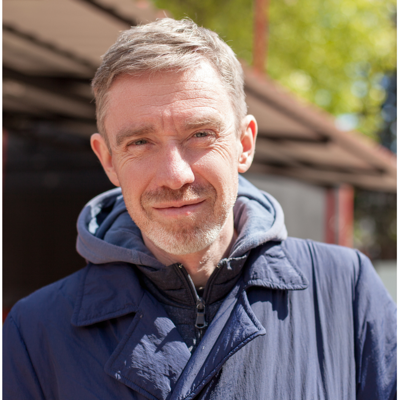
\includegraphics[width=3cm,height=3cm]{figures/persona-carlos}};
        \end{scope}
        \draw[rounded corners=8pt, black!30] (0,0) rectangle (3,3);
    \end{tikzpicture}
\end{minipage}\hfill
\begin{minipage}[c]{0.72\textwidth}
    {\textbf{Carlos Gómez}} \\
    55 años - Se dedica a hacer fletes - Quilmes, Buenos Aires
\end{minipage}

\begin{itemize}[leftmargin=2em]
  \item\textbf{Contexto y rol respecto al producto o sistema} \hfill \\
    Tiene un camión de mudanzas y actualmente consigue sus clientes a través de conocidos o por grupos de Facebook. No tiene app propia ni referencias visibles.
  \item\textbf{Objetivos al usar el producto} \hfill \\
    Quiere recibir alertas estructuradas de cargas grandes y mudanzas, con información clara del origen, destino y pago antes de confirmar.
  \item\textbf{Frustraciones y obstáculos actuales} \hfill \\
    Al depender de referencias personales, su demanda es irregular y no puede mantener un flujo constante de trabajo. Además suele encontrarse limitado a su zona de influencia, lo que restringe su capacidad de ampliar la clientela.
  \item\textbf{Comportamientos y hábitos relevantes} \hfill \\
	No le importa el desvío porque se desplaza específicamente para cada pedido a demanda del cliente.
  \item\textbf{Cita representativa} \hfill \\
    \textit{"Quisiera tener una forma más estructurada de conseguir clientes para mis fletes y al mismo tiempo generar un espacio con referencias que otros potenciales clientes puedan consultar para confiar en mi servicio."}
\end{itemize}
